\chapter{Results}
\label{chap:results}


\section{Preliminary Data Analysis}

In this section we report the preliminary data analysis that we have done in order to better understand the problem and select the most appropriate methods. However, due to privacy reasons we cannot expose private information regarding the players or the game and as a consequence some of the values have been standardized while others have been completely hidden. The purpose of this section is not to illustrate the underling data but is to give an idea of how we approached the problem and also make it clearer some of the choices that we have done.

For each game match that we tracked, we collected 11 different features. The features collected regard the match itself and do not concern with personal information of the players, e.g. gender, age or country. Furthermore, also the identifiers used to link the matches have been anonymised in a way that it is not possible to go back to the real players. Subsequently, we expanded these features computing the following statistics:
\begin{itemize}
    \item[--] minimum 
    \item[--] maximum 
    \item[--] average 
    \item[--] standard deviation
    \item[--] first quartile
    \item[--] median
    \item[--] third quartile
\end{itemize}

As a result we can describe each player with 77 features. Then, the successive step was to pre-process and clean the data to retain only relevant information. We removed duplicates or data that contained errors. Furthermore, we removed those features that had variance equal to zero meaning that the value was the same for all the players. For example, when we focused on the players that reached level 2500, the maximum number of stars for every player was 3. This means that the tracked players in at least one of the training levels have reached a 3 stars score. Since this features does not give any contribute to the player analysis we removed it.
Then, we handled the missing values. We decided to use different techniques based on the type of missing value. In this research we used deletion, imputation with mean value and linear interpolation. Subsequently we standardized all the data computing the z-score as follows: 
\begin{equation}
    \text{z-score} = \frac{x - \mu}{\sigma} \text{,}
\end{equation}
where $x$ is the feature, $\mu$ is the mean and $\sigma$ is the standard deviation of the considered feature $x$. After, we removed the outliers. We considered as outliers all the data that had a standard deviation that was higher than +10 or lower than -10. Finally, since most of the remained features were highly correlated we computed the correlation matrix and removed those features that had a correlation with any other feature that was higher than 0.9. As a result each player was described with 25 different features. 

After pre-processing the data, the first analysis we did was the eigenvalue and eigenvector decomposition of the matrix containing the players and their features. Figure \ref{fig:eig} illustrates the eigenvalue decomposition of the player features matrix. The eigenvalues are plotted in decreasing order. The figure shows that three eigenvalues have a value that is significantly higher than the others. 
\begin{figure}[!h]
  \centering
    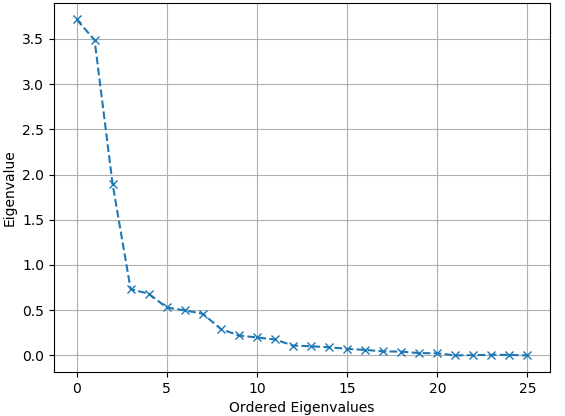
\includegraphics[width=0.6\textwidth]{masters-thesis-master/masters-thesis/contents/04_results/pre_data_analysis/eig_ord.png}
    \caption{Eigenvalue decomposition of the player matrix. The x-axis represents the 25 different features ordered by their eigenvalues in decreasing order and the y-axis the corresponding eigenvalues.}
    \label{fig:eig}
\end{figure}
To better visualize the implications of this analysis we illustrate in Figure \ref{fig:eig_var} the individual explained variance of each feature with the histogram and the cumulative explained variance with the blue line.
\begin{figure}[!h]
  \centering
    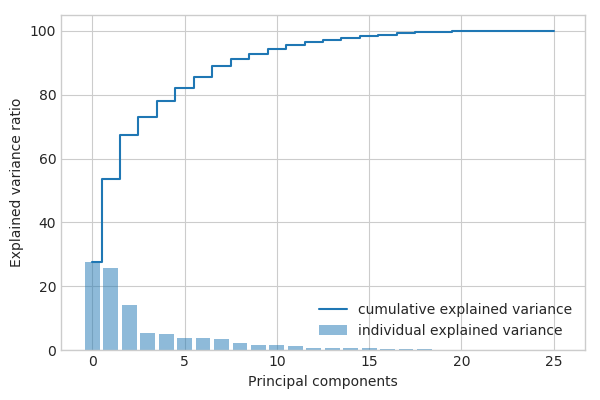
\includegraphics[width=0.6\textwidth]{masters-thesis-master/masters-thesis/contents/04_results/pre_data_analysis/eig_var.png}
    \caption{Individual explained variance of each feature illustrated with the histogram and cumulative explained variance illustrated by the blue line.}
    \label{fig:eig_var}
\end{figure}
We observed that only three player features are sufficient to explain almost 70\% of the overall variance. As a consequence, we performed \acf{PCA} on our data using three principal components. We then computed the sum of the absolute values of each coefficients for the 25 player features and scaled each coefficient by the explained variance ratio of the corresponding component. By ordering the features based on the computed values we can observe which feature contributes the most if we want to reconstruct the data into the original space with 25 dimensions. Results showed that the average player's \acs{sr} is the most important feature. Furthermore, we observed that the average amount of booster and the number of levels played are also important features to reconstruct the data. This motivates the choices that we made in the clustering simulated strategy approach where we decided to use these three features to describe the players. 
Furthermore we also experimented to perform a \acs{PCA} with 10 components since in this way we are able to explain almost 93\% of the overall variance. However as visible in Figure \ref{fig:pca_10} we observe that the explained variance ratio significantly decreases after the third component. 
\begin{figure}[!h]
  \centering
    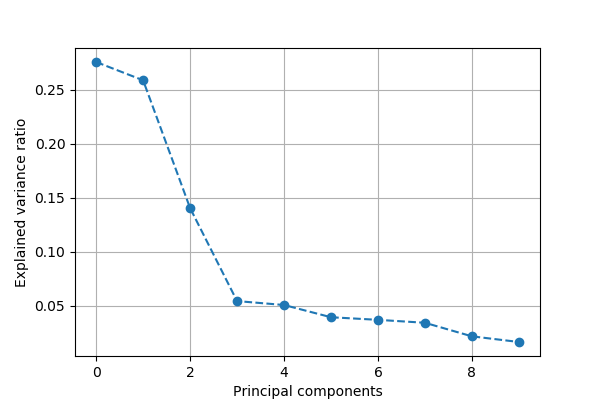
\includegraphics[width=0.6\textwidth]{masters-thesis-master/masters-thesis/contents/04_results/pre_data_analysis/pca10.png}
    \caption{Explained variance ratio of the 10 components obtained with principal component analysis.}
    \label{fig:pca_10}
\end{figure}
Furthermore, by computing again the importance of each feature we obtained similar results to the analysis with three principal components.

Another analysis that we performed was to understand how many clusters of players are present in the data. We ran the k-means algorithm on the cleaned player data with different number of clusters $k$ and used the "elbow criterion" to analyze the result. Figure \ref{fig:k_means_players} illustrates that between four and eight are reasonable numbers of player clusters. This motivates our choice of generating six agents that simulate six different groups of players.  
\begin{figure}[!h]
  \centering
    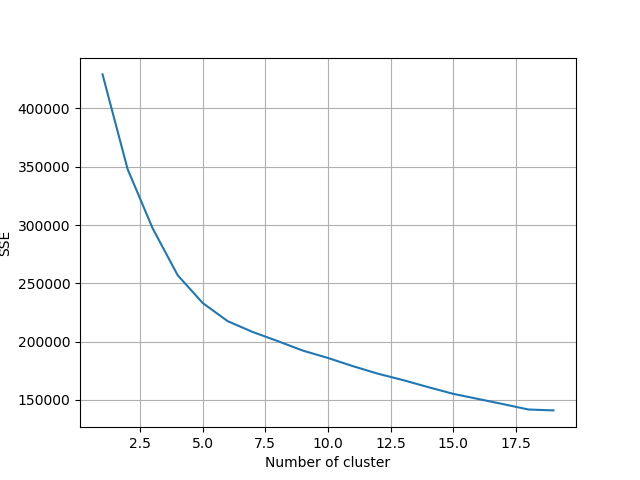
\includegraphics[width=0.6\textwidth]{masters-thesis-master/masters-thesis/contents/04_results/pre_data_analysis/k_means_players.png}
    \caption{Elbow criterion to understand how many player cluster are present in the data describing the players with 25 features.}
    \label{fig:k_means_players}
\end{figure}
Furthermore we performed an analysis of the levels in the game. We observed the distribution of the average players' \acs{sr} and their frequency. However, these data cannot be published.  
Finally, we performed an analysis of the distributions of the player features along the 2500 training levels. In the clustering player approach we decided to use the distribution of the standardized \acs{sr} to describe each player. We also experimented with the distribution of the standardized amount of boosters and the distribution of the standardized maximum number of stars. In Figure \ref{fig:boosters_distrib} we illustrate the six generated centroids obtained by clustering the booster distributions. 
\begin{figure}[H]
  \centering
    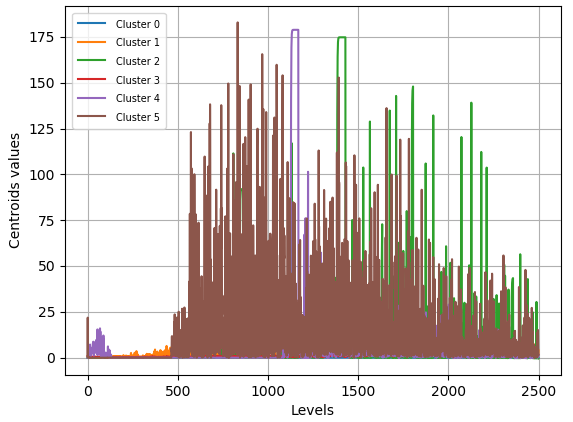
\includegraphics[width=0.6\textwidth]{masters-thesis-master/masters-thesis/contents/04_results/pre_data_analysis/boosters_distrib.png}
    \caption{Centroids obtained by the k-means clustering algorithm on the standardized amount of booster distributions.}
    \label{fig:boosters_distrib}
\end{figure}
However, clustering by the standardized amount of booster generated very unbalanced clusters, some of them containing only a single data point representing an outlier. Furthermore, the generated clusters were not interpretable and as a consequence we decided to not continue into this direction. Clustering by the maximum number of stars generated more balanced clusters. However, since the number of stars can assume only three different values we decided to use the players' \acs{sr} to represent the performances of the players in the game. 

\section{Player Modeling}
We illustrate in the following section the results of the two experimented approaches regarding the modeling of the players and the creation of the various agents that simulate different strategies.


\subsection{Clustering Players Approach}
We represented each player with a one dimensional array containing all his $2,500$ standardized success rates $\rho_i$ on the training levels. However, some players have missing SR for various reasons. The missing data points represent $5.16\%$ of the total number of players' \acs{sr}. In order to have comparable players' \acs{sr} distributions, we reconstructed the missing values using linear interpolation.
Figure \ref{fig:player_distribution} shows two examples of standardized players' SR distributions over the training levels. In order to select the number of player clusters $k$, we used the elbow criterion. By looking at the plot of the SSE against several numbers of $k$, as illustrated in Figure \ref{fig:select_k}, we decided to group the players into six different clusters. 

\begin{figure}[h]
  \centering
  \subfloat[]{
    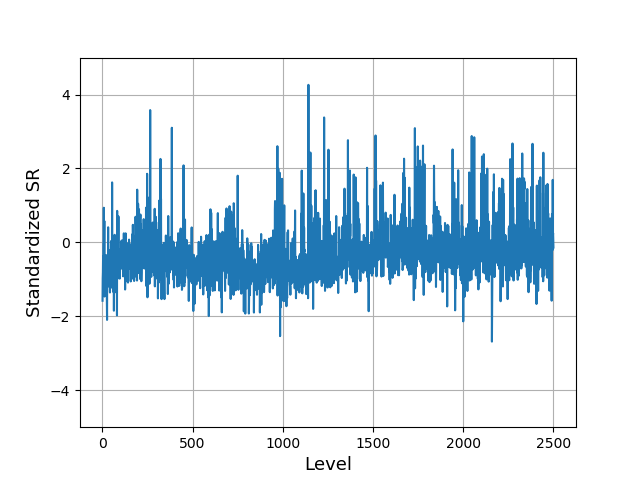
\includegraphics[width=0.45\textwidth]{masters-thesis-master/masters-thesis/contents/04_results/clustering_players_images/one_player_sr_distribution.png}
    \label{fig:player_distribution:a}
    }
  \subfloat[]{
    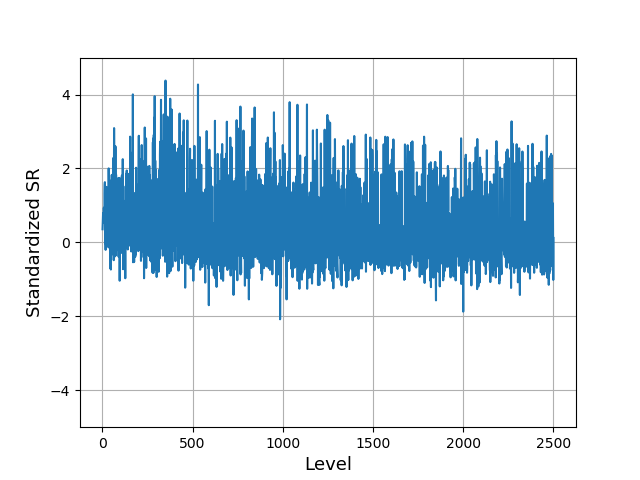
\includegraphics[width=0.45\textwidth]{masters-thesis-master/masters-thesis/contents/04_results/clustering_players_images/one_player_sr_distribution_2.png}
    \label{fig:player_distribution:b}
    }
    \caption{Two examples of standardized players' SR distributions over the levels in range [1, 2500]. 
    }
    \label{fig:player_distribution}
\end{figure}
\begin{figure}[h!]
  \centering
    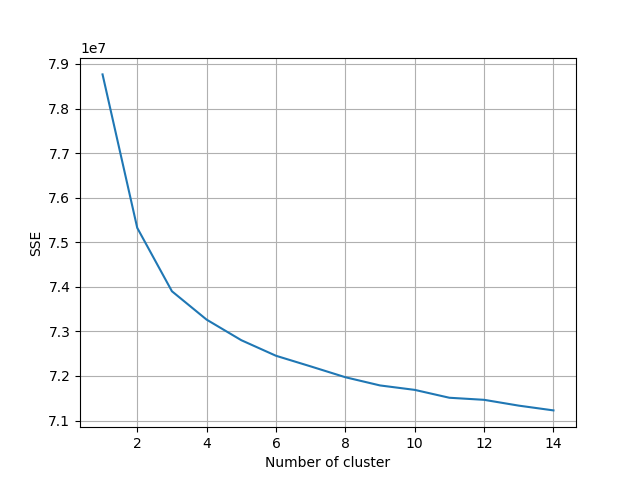
\includegraphics[width=0.6\textwidth]{masters-thesis-master/masters-thesis/contents/04_results/clustering_players_images/select_k.png}
    \caption{Elbow line used to select the number of clusters $k$. On the x-axis various numbers of $k$ while on the y-axis the SSE of the corresponding generated clusters. The plot shows that reasonable values of $k$ are between 3 and 8.}
    \label{fig:select_k}
\end{figure}
\noindent
Subsequently, we applied k-means to the players' SR distributions. Figure \ref{fig:k_means} shows the centroids of the generated clusters. 
\begin{figure}[h!]
  \centering
    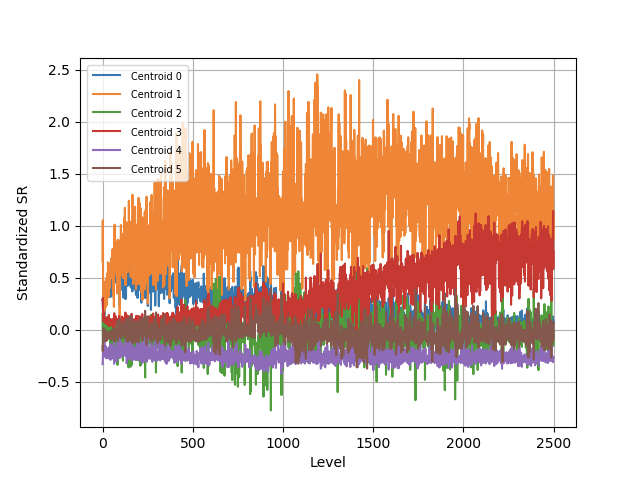
\includegraphics[width=0.6\textwidth]{masters-thesis-master/masters-thesis/contents/04_results/clustering_players_images/centroids_6_clusters.png}
    \caption{Centroids of the 6 generated clusters. The x-axis represents the training levels while on the y-axis the standardized SR. Centroid 0, in blue, represents players with decreasing standardized SR, centroid 1, in orange, represents players with high standardized SR, centroid 2, in green, represents players with average standardized SR, centroid 3, in red, represents players with increasing standardized SR, centroid 4, in purple, represents players with low standardized SR and finally, centroid 5, in brown, represents players with average standardized SR but with less variance compared to centroid 3. [This image is better viewed in colors].
    }
    \label{fig:k_means}
\end{figure}
By looking at the centroids, we can qualitatively describe the six different types of players represented by each cluster. Players in cluster 1 (orange) show a consistently high standardized SR and the cluster can therefore represents very good players. On the contrary, players in cluster 4 (purple), show a very low standardized SR distribution and the cluster can therefore represents less skilled players. 
Players in cluster 0 (blue) show a decreasing standardized SR and the cluster can therefore represents players that encounter difficulties in progressing the game. On the contrary, players in cluster 3 (red), show an increasing standardized SR and the cluster can therefore represents players that learn good strategies over time. Finally, players in cluster 2 (green) show a standardized SR distribution close to the average as well as players in cluster 5 (brown), but with slightly less variance over the levels.
Since k-means generates clusters with different sizes, in Table \ref{tab:clusters_features} we reported the number of players in each cluster. Note that cluster 1 contains only 2\% of the players, indicating the possibility that these players are simply outliers. To understand if the variability in the standardized players' SR distribution has an impact on the obtained clusters, we tried to cluster the levels into few buckets based on their difficulty and then represent each player with his average standardized SR distribution over the buckets. Since we obtained similar player clusters we decided to use the simplest approach avoiding to introduce a second clustering step on the levels.


\begin{table}[h]
    \centering
    \small
    \caption{Player clusters}
    \begin{tabular}{c l c S}
    \toprule
    Cluster \# & Color & \text{\# of Players} & \text{\% of Players} \\
    \midrule
    0 & blue & 3460 & 10.65  \\
    1 & orange & 652 & 2.00 \\
    2 & green & 7042 & 21.68  \\
    3 & red & 2581 & 7.95 \\
    4 & purple & 8958 & 27.58  \\
    5 & brown & 9786 & 30.13 \\
    \bottomrule
    \end{tabular}
    \label{tab:clusters_features}
\end{table}

\subsection{Clustering Simulated Strategies Approach}

In this approach we decided to add other two player features: the standardized mean amount of booster $\bar{\beta}$ and the number of levels played $l$ during the tracking period. Furthermore, instead of using the distribution of the \acs{sr} along the levels, we aggregated the values to have a single measure $\bar{\rho}$, that represents the overall skill of the player. Then, we let the network detect the relationship between these features and the performed move. After training the \acs{CNN}, we predicted on a validation set of 10,000 states with 125 different input player feature combinations. We generated all the possible combinations using the 5th, 25th, 50th, 75th and 95th percentiles of each player feature. The moves predicted by each agent are then considered as a sort of explicit representation of the simulated strategy of the agent. Clustering the simulated strategies we selected six agents that maximized the difference in the predicted moves. Results showed that the 25th and the 75th percentiles were never used by any of the obtained agents. This is reasonable since the player features are real numbers and extreme values lead to more diverse strategies. As a consequence we experimented repeating the clustering only with the 5th, 50th, and 95th percentiles of each player feature. Figure \ref{fig:hierarchical_clustering} shows the dendogram generated by hierarchical clustering. 
\begin{figure}[h!]
  \centering
    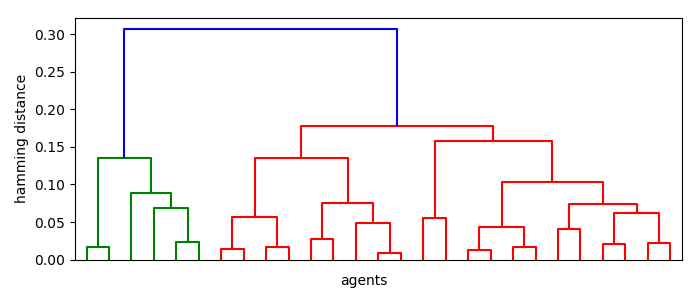
\includegraphics[width=0.6\textwidth]{masters-thesis-master/masters-thesis/contents/04_results/Player_Modeling/Sim_strategies/Plots/hierarchical.png}
    \caption{Dendogram illustrating the differences in the simulated strategies of 27 different agents. The x-axis represents the 27 different generated agents with different combinations of the standardized mean success rate $\bar{\rho}$, the standardized mean amount of boosters $\bar{\beta}$ and the number of different levels played $l$. The y-axis represents the percentage of moves that the agents predict differently. 
    }
    % Each agent share the same network but uses different player features as input. The player features on the x-axis are abbreviated as follows: "bo" means the standardized mean amount of boosters $\bar{\beta}$, "di" means the standardized number of different levels played $l$ while "sk" means skill and represent the standardized mean success rate $\bar{\rho}$.
    \label{fig:hierarchical_clustering}
\end{figure}
\noindent
It shows that most of the agents have very similar predictions, however the six most different agents have a difference in the simulated strategies of at least 13\%. This means that by changing the player features the network predicts differently. 
Table \ref{tab:agents_generated_sim_strategies} shows the selected agents, their player features and a possible interpretation of the simulated types of players. The selected agents are the ones that on each of the six major clusters have a distance to their merged cluster that is the maximum compared to the other agents in the same cluster. As distance measure we used the hamming distance between the simulated strategies. The hamming distance represents the percentage of moves that the compared agents predict differently. We can observe that the two most diverse agents select different moves 31\% of the time.
\begin{table}[h]
    \centering
    \small
    \caption{Agents generated by clustering simulated strategies} 
       \begin{tabular}{l S c S l }
    \toprule
    
    Agent & \text{Skill ($\bar{\rho}$)} &  Levels played ($l$) & \text{Boosters ($\bar{\beta}$)} & Description \\

    \midrule
    Agent 0 & -0.76  & 241 & -0.06   & less skilled player \\ 
    Agent 1 & -0.76  & 69  & 1.51    & less skilled occasional booster player \\ 
    Agent 2 & 0.96   & 927 & -0.37   & skilled regular non-booster player \\ 
    Agent 3 & 0.96   & 927 & 1.51    & skilled regular booster player \\ 
    Agent 4 & 0.05   & 241 & 1.51    & booster player \\ 
    Agent 5 & 0.96   & 69  & -0.37   & skilled occasional non-booster player \\ 
   % Baseline & \text{-}     & \text{-}   & \text{-}       & average strategy  \\ 

    
    \bottomrule
    \end{tabular}
    \label{tab:agents_generated_sim_strategies}
\end{table} 


\section{CNNs Training and Prediction}

Except for the input size, we used the same network architecture for the two experimented approaches. Regarding the clustering players approach, Table \ref{tab:Top1_training_test_accuracy} reports the top-1 accuracy, while Table \ref{tab:Top3_training_test_accuracy} reports the top-3 accuracy of each agent. 
\begin{table}[b]
    \centering
    \small
    \caption{Clustering players. Top-1 training and test accuracy} 
    
    \begin{tabular}{l c c c c c c c}
    \toprule

    Data set & Agent 0 & Agent 1 & Agent 2 & Agent 3 & Agent 4 & Agent 5 & Baseline \\
    
    \midrule
    Training data & \textbf{52.97} & 47.46 & 48.77 & 46.39 & 49.10 & 51.78 & 49.74\\
    \hline
    Test cluster 0 data & \textbf{51.93} & - & - & - & - & - & 51.16 \\
    Test cluster 1 data & - & \textbf{47.06} & - & - & - & - & 46.02\\
    Test cluster 2 data & - & - & \textbf{53.03} & - & - & - & 51.97\\
    Test cluster 3 data & - & - & - & \textbf{46.78} & - & - & 45.54\\
    Test cluster 4 data & - & - & - & - & \textbf{51.95} & - & 51.85\\
    Test cluster 5 data & - & - & - & - & - & \textbf{52.89} & 52.49\\
    Test baseline data & 50.11 & 49.52 & \textbf{50.56} & 50.14 & 49.86 & 50.53 & 50.11\\
    \bottomrule
        
    \end{tabular}

    \label{tab:Top1_training_test_accuracy}
\end{table}
With bold we indicate the agent with the best accuracy on each data set. Each row represents a different data set. The first row represents the training accuracy of each agent on its own last mini-batch (consisting of 2048 examples). The remaining rows represent the test accuracy on different test data sets (each one consisting of 100,000 examples). By looking at the accuracy on the test data sets, we observed that in both the top-1 and top-3 accuracy, each agent better represents the players in its cluster compared to the baseline approach. This indicates that the \acs{CNN} model is able to learn different policies by changing the input data used during training. However, we observed that there is only a small difference between the prediction accuracy of the agents and the baseline. This is explained by the fact that we ran experiments with thousands of different players. As a consequence, even if we divide the data, each cluster contains examples from many different players and the \acs{CNN} learns the average strategy of the players on each cluster. Combining data of such a large number of players reduces the differences in the strategies learnt. Furthermore, we noted that the baseline accuracy is different on each data set. This confirms that players in different clusters select moves with different strategies and the baseline agent is not specialized to predict any of them. Furthermore, also the agents show different accuracy. A possible explanation is that some players select moves that are more predictable than other players. For example, players in cluster 2, select moves that are more easily predictable by the \acs{CNN}-based model than any other player cluster since the agent 2 performed better than any other agent in the top-1 accuracy.
Nevertheless, all the agents showed a similar training progression and as an example, in Figure \ref{fig:nn_train} we illustrate the training process of two of them.  Finally, if we use the agents to predict on the same game boards, on average they disagree 30\% of the times, meaning that approximately one third of the times they select different moves between each other. This confirms once again that we learned different player strategies. Note that the prediction accuracy of the model does not directly relate to their performances in the game. An agent can be very good in predicting the players that simulates but if the moves performed by that players are bad, the agent will perform poorly when playing the game. With a similar reasoning, even the improvement of the agents' accuracy compared to the baseline agent on each player cluster does not necessary mean that the agents are better than the baseline during gameplay. The tables only shows that each agents better predict the players that simulate compared to the baseline agent and that different player cluster use different strategies.
\begin{table}[t]
    \centering
    \small
    \caption{Clustering players. Top-3 training and test accuracy} 
    
    \begin{tabular}{l c c c c c c c}
    \toprule

    Data set & Agent 0 & Agent 1 & Agent 2 & Agent 3 & Agent 4 & Agent 5 & Baseline \\
    
    \midrule
    Training data & 82.35 & 77.15 & 80.40 & 77.35 & 81.24 & \textbf{82.82} & 81.01\\
    \hline
    Test cluster 0 data & \textbf{82.79} & - & - & - & - & - & 82.46 \\
    Test cluster 1 data & - & \textbf{78.26} & - & - & - & - & 77.50\\
    Test cluster 2 data & - & - & \textbf{83.63} & - & - & - & 82.99\\
    Test cluster 3 data & - & - & - & \textbf{77.73} & - & - & 76.74\\
    Test cluster 4 data & - & - & - & - & \textbf{83.68} & - & 83.45\\
    Test cluster 5 data & - & - & - & - & - & \textbf{83.75} & 83.56\\
    Test baseline data & 81.47 & 81.11 & \textbf{81.96} & 81.80 & 81.52 & 81.52 & 81.56\\
    \bottomrule
        
    \end{tabular}
    \label{tab:Top3_training_test_accuracy}
\end{table} 
\begin{figure}        
\centering
    \subfloat[]{%Top-1 training accuracy
    \resizebox{0.30\textwidth}{!}{%
\begin{tikzpicture}[]

\begin{axis}[
xlabel={Step},
ylabel={Top-1 accuracy},
legend style={at={(0.96,0.25)}}
]   
    %HU
    \addplot[
    black,
    ]
    table [x=Step, y=Value, col sep = comma]
    {contents/04_results/gameplay_simulation/data/cluster1_top1.csv};

    
    % HF
    \addplot[
    cyan,
    ]
    table [x=Step, y=Value, col sep = comma] {contents/04_results/gameplay_simulation/data/cluster2_top1.csv};
    
    \legend{Agent 1,Agent 2}
    

\end{axis}

\end{tikzpicture}
}
    \label{fig:train_acc_1}
    }
    \subfloat[]{%Top-3 training accuracy
    \resizebox{0.30\textwidth}{!}{%
\begin{tikzpicture}[]

\begin{axis}[
xlabel={Step},
ylabel={Top-3 accuracy},
legend style={at={(0.96,0.25)}}
% scaled x ticks={real:28000},
% xtick scale label code/.code={}
]   
    %HU
    \addplot[
    black,
    ]
    table [x=Step, y=Value, col sep = comma] {contents/04_results/gameplay_simulation/data/cluster1_top3.csv};
    
    % HF
    \addplot[
    cyan,
    ]
    table [x=Step, y=Value, col sep = comma] {contents/04_results/gameplay_simulation/data/cluster2_top3.csv};

    \legend{Agent 1,Agent 2}

\end{axis}

\end{tikzpicture}
}
    \label{fig:train_acc_3}
    }
    \subfloat[]{%Batch loss
    \resizebox{0.285\textwidth}{!}{%
\begin{tikzpicture}[]

\begin{axis}[
xlabel={Step},
ylabel={Batch loss}
% scaled x ticks={real:28000},
% xtick scale label code/.code={}
]   
    %HU
    \addplot[
    black,
    ]
    table [x=Step, y=Value, col sep = comma] {contents/04_results/gameplay_simulation/data/cluster1_loss.csv};
    
    % HF
    \addplot[
    cyan,
    ]
    table [x=Step, y=Value, col sep = comma] {contents/04_results/gameplay_simulation/data/cluster2_loss.csv};

    \legend{Agent 1,Agent 2}

\end{axis}

\end{tikzpicture}
}
    \label{fig:train_batch_loss}
    }
    \caption{Visualization of the training process for agents 1 and 2. Figure (a) illustrates the top-1 training accuracy, Figure (b) shows the top-3 training accuracy while Figure (c) illustrates the batch loss. }
    \label{fig:nn_train}
\end{figure}

Regarding the clustering simulated strategies approach, Table \ref{tab:top1_top3_training_test_accuracy} illustrates the top-1 and top-3 test and training accuracy. We reported the accuracy for both the network that uses the player features and the baseline. 
% Results showed that there is no substantial difference between the experimented approach and the baseline in terms of prediction accuracy, indicating that adding the player features as input does not significantly improve the power of the predictive model. However, 
The maximum disagreement between the generated agents is 31\%, meaning that the \acs{CNN} has learnt to play differently based on the values of the player features.
Finally, we observed that the test accuracy in the clustering player approach is higher than the test accuracy in the clustering simulated strategies approach. A possible explanation is that in the first approach we restricted our focus to players that finished all the training levels and the moves performed by these players are more predictable than the ones performed by random players.  
\begin{table}[h]
    \centering
    \small
    \caption{Clustering simulated strategies. Top-1 and top-3 training and test accuracy of the agent trained with player features and the baseline} 
        
    \begin{tabular}{c c c c }
    \toprule
    
    Data set & Accuracy & Player Features Agent & Baseline \\
    
    \midrule
    \multirow{2}{7em}{Training data} & Top-1 & \textbf{46.52} & 46.04 \\
    & Top-3 & 78.08 & \textbf{78.29} \\
    \hline
    \multirow{2}{7em}{Test data} & Top-1 & \textbf{46.28} & 46.11 \\
    & Top-3 & \textbf{78.01} & 77.82 \\
    \bottomrule
        
    \end{tabular}
    \label{tab:top1_top3_training_test_accuracy}
\end{table} 



\section{Players' SR Prediction}
Throughout this thesis, in order to not expose the actual values for privacy purposes, the players’ SR has been scaled by the difference between the maximum and the minimum \acs{sr} as described in Equation \ref{eq:scaled_sr}.
% The scaling is applied equally to all the players' SR. 
Note that the agents' SR have not been scaled and that on both the scaled players' SR and the agents' SR we applied a log transformation to obtain less skewed distributions.
% Furthermore, applying the log transformation causes the log of the agents' SR that are zero to become minus infinite. 
Furthermore, we used linear regression models to predict the log of the scaled players' SR when the agents' SR is greater than zero and the mean of the log of the scaled players' SR on training levels as a prediction when the agents' SR is zero. For comprehensibility, in the rest of the thesis we will refer to the log of the scaled players' SR as simply the players' SR and we will refer to the log of the agents' SR as simply the agents' SR. 

\subsection{Clustering Players Approach}

In order to validate our models we performed various tests.
First, we tested that there exists a statistical relationship in the training data between each agent's \acs{sr} and the players' \acs{sr} that each agent simulates. Since each agent uses only a single predictor, in Table \ref{tab:reg_analysis} we reported its coefficient and the regression statistics. We can observe that the p-values are all lower than 5\% meaning that is likely that changes in the predictor are related to changes in the response variable. In our case this means that changes in the agent's \acs{sr} are likely to be related to changes in the players' \acs{sr}. Note that each line in the table refers to a different linear model that correlates the agent's \acs{sr} with its corresponding players' \acs{sr}. 
\begin{table}[h]
    \centering
    \small
    \caption{Linear regression analysis between each agents' SR and its corresponding players' SR in the training data} 
       \begin{tabular}{l c c S c }
    \toprule
    
    Agent & coef. & std. err. & \text{t-stat.} & p-value \\
    
    \midrule
    Baseline & 0.696 &      0.006 &    120.84 &      0.00\\ 
    Agent 0 & 0.618  &     0.005  &   127.08  &     0.00\\ 
    Agent 1 & 0.317  &    0.004   &   71.55   &    0.00 \\
    Agent 2 & 0.668  &     0.006  &   105.54  &     0.00\\ 
    Agent 3 & 0.528  &     0.006  &    87.40  &     0.00\\ 
    Agent 4 & 0.800  &     0.006  &   124.90  &     0.00\\ 
    Agent 5 & 0.689  &     0.006  &   124.64  &     0.00\\ 
    
    
    \bottomrule
        
    \end{tabular}
    \label{tab:reg_analysis}
\end{table} 

Since we used linear regression models to predict the players' \acs{sr} we also need to ensure that the following assumptions are valid:
\begin{enumerate}
    \item Linearity of the relationship between dependent and independent variables
    \item Homoscedasticity of the errors
    \item Statistical independence of the errors
    \item Normality of the error distribution
\end{enumerate}

\begin{figure}[ht!]
  \centering
  \subfloat[]{%Players' SR vs predicted SR
    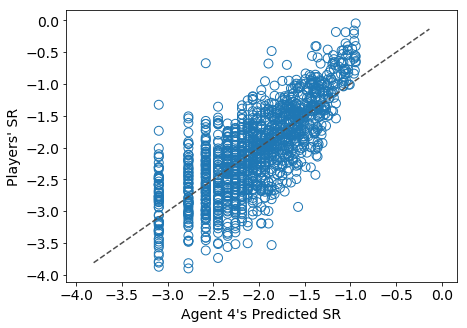
\includegraphics[width=0.31\textwidth]{masters-thesis-master/masters-thesis/contents/04_results/Player_Modeling/Clustering/plots/agent4_pred_obs.png}
    \label{fig:train_example_residuals:train_pred_obs}
    }
    \subfloat[]{%Agent 4's SR vs residuals
    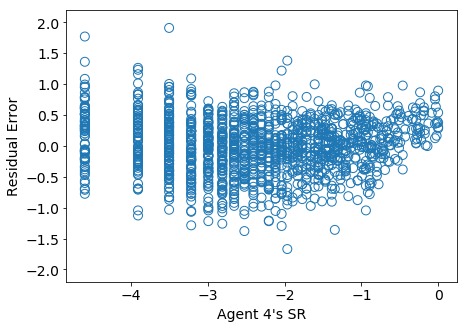
\includegraphics[width=0.31\textwidth]{masters-thesis-master/masters-thesis/contents/04_results/Player_Modeling/Clustering/plots/agent4_res_sr.png}
    \label{fig:train_example_residuals:train_sr}
    }
  \subfloat[]{%Levels vs residuals
    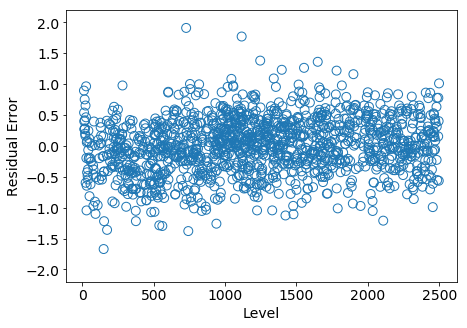
\includegraphics[width=0.31\textwidth]{masters-thesis-master/masters-thesis/contents/04_results/Player_Modeling/Clustering/plots/agent4_res_levels.png}
    \label{fig:train_example_residuals:train_levels}
    }
    
  \subfloat[]{%Residuals frequency
    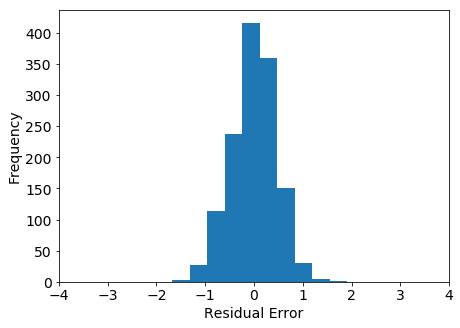
\includegraphics[width=0.31\textwidth]{masters-thesis-master/masters-thesis/contents/04_results/Player_Modeling/Clustering/plots/agent4_res_freq.png}
    \label{fig:train_example_residuals:train_frequency}
    }
  \subfloat[]{%Normal probability plot
    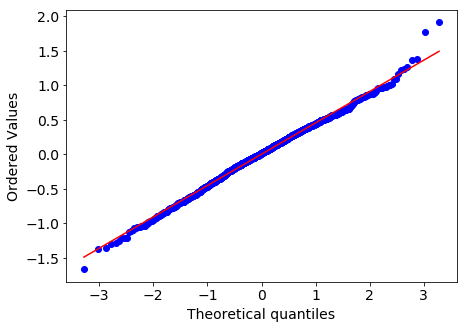
\includegraphics[width=0.315\textwidth]{masters-thesis-master/masters-thesis/contents/04_results/Player_Modeling/Clustering/plots/agent4_qq.png}
    \centering
    \label{fig:train_example_residuals:train_qq}
    }
    \caption{Plots validating the linear regression assumptions in the training data for agent 4. Figure (a) illustrates the linear relationship between the players' SR and the predicted players' SR, the black dashed line is the diagonal. Figure (b) shows the agent's SR against the residual errors while Figure (c) shows the levels against the residuals. Figure (d) shows the histogram of the residual errors and finally, Figure (e) shows the normal probability plot of the residuals.}
    \label{fig:train_example_residuals}
\end{figure}
\noindent
As an example, we check these assumptions for the linear regression model trained with agent 4's \acs{sr}. The same tests are performed with all the remaining linear models and the plots are illustrated in Appendix \ref{assamp_val}. Note, that these analysis are performed on the training data before using the linear models for prediction.
Plotting the agent 4's predicted \acs{sr} against the players' \acs{sr}, as illustrated in Figure \ref{fig:train_example_residuals:train_pred_obs}, we validated that exists a linear relationship between the dependent and the independent variables. Except for very high values of the agent's \acs{sr}, the data points are symmetrically distributed around the diagonal line. This implies that there is no major violation of the linear relationship assumption (1). 
Figure \ref{fig:train_example_residuals:train_sr} illustrates the agent's \acs{sr} against the residual errors. The variance of the errors seems to be fairly constant along the independent variable, except for very high agent's \acs{sr} where it seems to be lower. For completeness, we also checked that the variance of the errors is constant along the dependent variable and we obtained similar results. As a consequence, the variance of the errors does not significantly increase as a function neither of the predicted players’ \acs{sr} nor the agents’ \acs{sr}. However, the residual errors seem to be centered around zero only for values of the agent's \acs{sr} between -1 and -4. For very low or very high agent's \acs{sr} the errors are not centered around zero. More precisely, when the agent's \acs{sr} is very low or very high, the residual error is more likely to be positive, meaning that we underestimate levels that are very difficult or very easy for the agent. 
% On the contrary, when the agent's \acs{sr} is high, the residual error is likely to be negative, meaning that we overestimate levels where the agent performs well.
However, since the data points that violate the homoscedasticity assumption (2) are only a small number compared to the total number of training data points, we concluded that there is only a minor violation of this assumption.
In Figure \ref{fig:train_example_residuals:train_sr}, we can also observe that consecutive errors are not correlated, therefore there is no violation of the statistical independence of the errors assumption (3). Figure \ref{fig:train_example_residuals:train_levels} shows that the errors are equally distributed along the levels as well.
Figure \ref{fig:train_example_residuals:train_frequency} illustrates the histogram of the residual errors. We can notice that the histogram seems to represent a normal distribution. Finally, we checked against violation of the normal distribution of the errors assumption (4) by looking at the normal probability plot \cite{chambers_assessing_1983} illustrated in Figure \ref{fig:train_example_residuals:train_qq}. We can see that only a few points at both the tails of the theoretical quantiles do not follow the line.
As a result, we can say that there is no violation of the normal distribution of the errors assumption.  

\begin{figure}[h!]
  \centering
  \subfloat[]{%Players' SR against predicted SR
    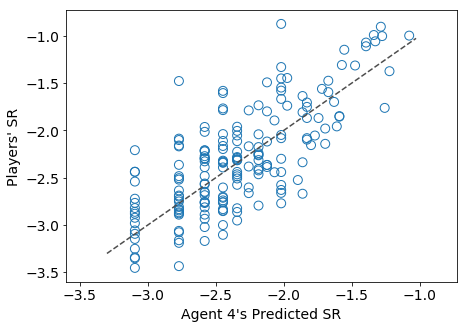
\includegraphics[width=0.45\textwidth]{masters-thesis-master/masters-thesis/contents/04_results/Player_Modeling/Clustering/plots/agent4_pred_obs_test.png}
    \label{fig:test_example_residuals:test_pred_obs}
    }
    \subfloat[]{%Agent 4's SR against residuals
    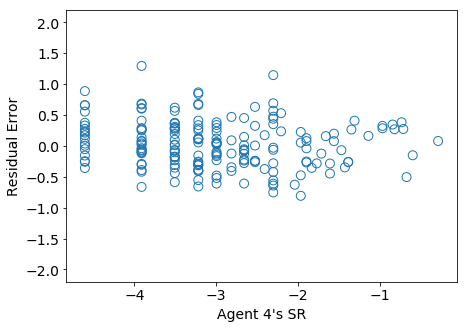
\includegraphics[width=0.45\textwidth]{masters-thesis-master/masters-thesis/contents/04_results/Player_Modeling/Clustering/plots/agent4_res_sr_test.png}
    \label{fig:test_example_residuals:test_sr}
    }
    
    \caption{Plots confirming the linear regression assumptions in the test data for the agent 4. Figure (a) illustrates the linear relationship between the players' SR and the predicted players' SR, the black dashed line is the diagonal. Figure (b) shows the agent's SR against the residual errors.}
    \label{fig:test_example_residuals}
\end{figure}
Similar conclusions can be derived for the other linear models with only few exceptions. The linear models trained with agent 1's and agent 3's \acs{sr} showed a small correlation between the levels and the residual errors. This is not surprising since the players that they simulate have a non-constant average \acs{sr} in the training data. This implies that for these two specific agents, adding the levels as a feature of the linear model could improve the performances. Moreover, the linear model trained with agent 1's \acs{sr} violates the normality of the error distribution assumption. However, this agent represent only 2\% of the total number of players and we knew that it could represents outliers or anomalous players. Since agent 1 and 3 represent only 9\% of the players in total, for practical purposes, a lower performance of the linear models for these agents is tolerable. Finally, similar plots for validating the assumptions with the baseline agent are reported in Appendix \ref{assamp_val}.
Subsequently, we use the fitted linear models to predict on test levels.
In Figure \ref{fig:test_example_residuals} we observe that the assumption we validated in the training data for the linear models still hold in the test data. More specifically, Figure \ref{fig:test_example_residuals:test_pred_obs} shows that there is a linear relationship between the agent's and the players' \acs{sr} in the test data while Figure \ref{fig:test_example_residuals:test_sr} shows that the residual errors are well distributed, not correlated and with a fairly constant variance.
In Figure \ref{fig:example_predictions}, as an example, we illustrate the \acs{sr} predictions of the players in cluster 4 for both the baseline and agent 4. The comparisons between the other agents and the baseline while predicting the remaining player clusters are reported in Appendix \ref{predictions_comparison}.
\begin{figure}[h!]
  \centering
  \subfloat[]{%Agent 4's predictions
    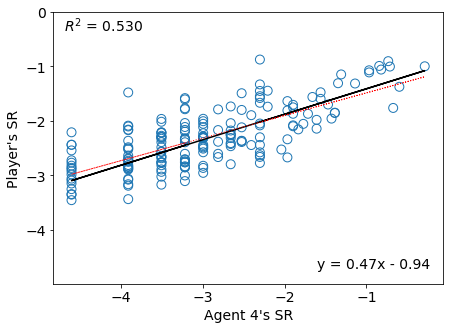
\includegraphics[width=0.45\textwidth]{masters-thesis-master/masters-thesis/contents/04_results/Player_Modeling/Clustering/plots/agent4_test_prediction.png}
    \label{fig:example_predictions:Agent 0's predictions}
    }
  \subfloat[]{%Baseline's predictions trained with all players
    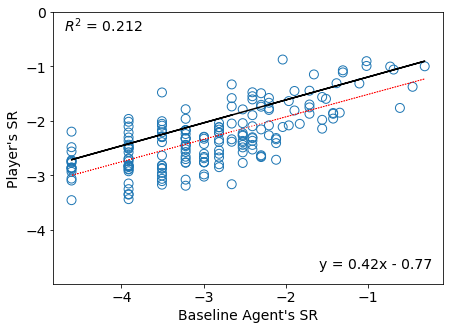
\includegraphics[width=0.45\textwidth]{masters-thesis-master/masters-thesis/contents/04_results/Player_Modeling/Clustering/plots/baseline4_test_prediction.png}
    \label{fig:example_predictions:Baseline agent's predictions}
    }
    
    \subfloat[]{%Baseline's predictions trained with players in cluster 4
    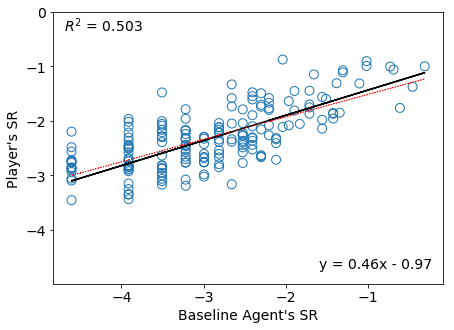
\includegraphics[width=0.45\textwidth]{masters-thesis-master/masters-thesis/contents/04_results/Player_Modeling/Clustering/plots/baseline4_test_pred_in_4.png}
    \label{fig:example_predictions:Baseline agent's predictions in 4}
    }
    \caption{Agent 4's and baseline's predictions for the success rate of players in cluster 4. Figure (a) illustrates the agent 4's predictions while Figures (b) and (c) show the predictions obtained from the baseline's SR. The baseline predictions in (b) are obtained training the baseline linear model to predict the average \acs{sr} of the players. The baseline predictions in (c) are obtained training the baseline linear model to predict the \acs{sr} of the players in cluster 4. In each graph, the black line shows the linear regression model while the red dashed line shows the ideal linear model. In the top left corner we illustrate the $R^2$ measure of the fitted regression model. In the bottom right corner of the graph we report the equation of the line obtained by the linear regression model.}
    \label{fig:example_predictions}
\end{figure}
We observe that the linear model fitted with the agent 4's \acs{sr} significantly outperforms the baseline in predicting the \acs{sr} of players in cluster 4. Moreover, we observe that the baseline approach systematically overestimates these players. This is explained by the fact that cluster 4 represents players which have a \acs{sr} distribution that is consistently under the average value. Similar reasoning can be done looking at the others agents' predictions compared to the baseline. Furthermore, Figure \ref{fig:example_predictions:Baseline agent's predictions in 4} shows that even if we train the baseline agent to predict the \acs{sr} of players in cluster 4 instead of predicting the average \acs{sr} between all the players, the prediction performances remain lower than those of agent 4. This confirms that the \acs{sr} of players in cluster 4 are more correlated to the \acs{sr} of agent 4 rather then the \acs{sr} of the baseline agent. However, if we train the baseline agent to predict the \acs{sr} of players in cluster 4 the difference with our approach in terms of \acs{sr} predictions is small. This suggest that after clustering the players, using only the baseline agent to predict each player cluster \acs{sr} could be a trade-off between computational requirements and prediction accuracy. 

Table \ref{tab:prediction_analysis} reports the MAE, MSE and adjusted R-squared computed on each player cluster. 
\begin{table}[b]
    \centering
    \small
    \caption{Analysis of the linear regression models while predicting on test data sets and comparison with the baseline agent} 
       \begin{tabular}{l c c c c S S }
    \toprule
    
    & \multicolumn{2}{c}{MAE} & \multicolumn{2}{c}{MSE} & \multicolumn{2}{c}{Adj R-squared} \\
    \cmidrule(r){2-3} 
    \cmidrule(r){4-5}
    \cmidrule(r){6-7}
    
    Players in & Agent & Baseline & Agent & Baseline & \text{Agent} & \text{Baseline} \\
    
    \midrule
    Cluster 0 & 0.27 & 0.34  &    0.12 &     0.19   &   0.47  &   0.12   \\ 
    
    Cluster 1 & 0.34 & 0.85 &    0.18 &     0.87  &   -0.27  &   -5.26  \\ 
    
    Cluster 2 & 0.33 & 0.34 &    0.16  &     0.17  &   0.34 &   0.30 \\ 
    
    Cluster 3 & 0.40 & 0.91 &    0.22 &     0.94  &   -0.99 &   -7.75 \\ 
    
    Cluster 4 & 0.31 & 0.41  &    0.15 &     0.26  &   0.49 &   0.13 \\ 
    
    Cluster 5 & 0.30  & 0.31  &    0.14 &     0.16  &   0.50 &   0.44  \\ 
    
    \bottomrule
        
    \end{tabular}
    \label{tab:prediction_analysis}
\end{table}
Note that on each row the "agent" columns describe a different agent, the one trained with the corresponding player cluster. For example, we never use agent 1 to predict the \acs{sr} of players in different clusters from cluster 1. On the contrary, the baseline columns indicate always the same baseline agent used to predict the \acs{sr} of players in all the defined clusters. We can observe that each linear model, compared to the baseline, better represents, in terms of \acs{sr} predictions on test levels, the players that the agent simulates. Note that the adjusted R-squared is 1 in the ideal case where the line perfectly fits all the data points but it does not have a lower bound. This means that as the linear model get worse, the adjusted R-squared value can become negative and it can decrease indefinitely. A boxplot illustrating the residual errors of the agents and the baseline on each player cluster is shown in Figure \ref{fig:boxplot}.
\begin{figure}[t]
    \centering
    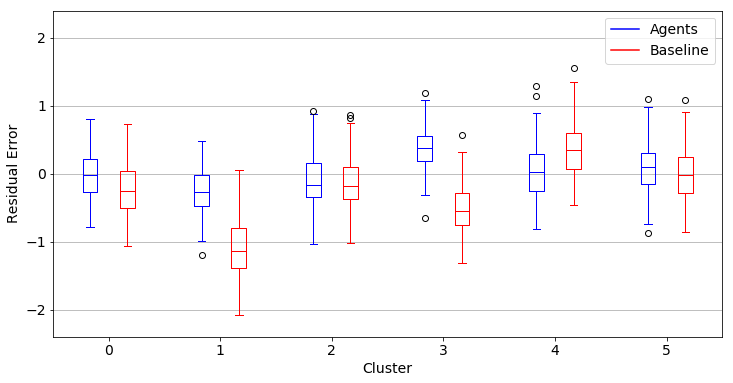
\includegraphics[width=0.6\textwidth]{masters-thesis-master/masters-thesis/contents/04_results/Player_Modeling/Clustering/plots/boxplot.png}
    \caption{Boxplot comparing agent's and baseline's residual errors. For each player cluster illustrates the distribution of the residual errors of the agent representing the cluster, in blue on the left, and the baseline approach, in red on the right.}
    \label{fig:boxplot}
\end{figure}
It shows that the agents have an error closer to zero and a lower variance, confirming that they can better predict the players' \acs{sr} that they simulate compared to the baseline.


Finally, in order to compare our approach with the baseline approach and answer our research question we combined the agents' predictions to obtain a single measure. The linear combination of the six predictions, as defined in \ref{combination}, is based on the percentage of players that each agent represents. Table \ref{tab:prediction_performance_linear} reports the evaluation of our approach compared to the baseline. The clustering players approach reduced the prediction MAE from 0.30 to 0.26 with an improvement of 13\% and reduced the prediction MSE from 0.13 to 0.10 with an improvement of 23\%. In the table we also reported the 95\% confidence interval of the mean. We ran a paired t-test to check that the mean difference between the absolute errors per each test level is different from zero. We decided to use a paired t-test because the two approaches are tested on the same levels and we want to remove the variability in the errors that has not been completely removed by the linear regression models due to the minor violation of the homoscedasticity assumption. The paired t-test increases the statistical power of our analysis because it removes the between-level variability. If a level is too difficult, the difference between the approaches does not have to be large even if the error is big. As a result, we obtained a two-tailed p-value of 0.04\%. Since it is lower than 5\% we rejected the hypothesis of no difference between the absolute errors of the two approaches. For completeness, we ran a two-sided t-test to check that the two approaches have a statistically different \acs{MAE}. Since we obtained a p-value lower than 5\%, we can reject the null hypothesis of identical average scores. Similar results were obtained for the \acs{MSE}. As a consequence, we have strong evidence that the new approach outperforms the baseline approach. The MAE is the metric that for practical purposes we consider most important between the two. We prefer to have few wrong predictions and frequent accurate predictions rather than constantly fairly accurate predictions. This because human testing is still worth when concerning subjective or qualitative measurements like fun or player experience and if applied in conjunction with our approach, it can easily detect highly wrong predictions.
\begin{table}[h!]
    \centering
    \small
    \caption{Clustering players. Overall linear regression performance measures} 
       \begin{tabular}{l c c}
    \toprule
    
    Approach  & MAE & MSE \\ % & Adj R-squared
    
    \midrule
    Baseline            & 0.30 $\pm$ 0.03  & 0.13 $\pm$ 0.02  \\ % &   0.43 
    Clustering players  & 0.26 $\pm$ 0.03  & 0.10 $\pm$ 0.02  \\ %  &   0.56
    

    \bottomrule
        
    \end{tabular}
    
    
    %   \begin{tabular}{l c c c c}
    % \toprule
    
    % & \multicolumn{2}{c}{MAE} & \multicolumn{2}{c}{MSE} \\
    % \cmidrule(r){2-3} 
    % \cmidrule(r){4-5}
    % Approach  & Mean & Std err & Mean & Std err \\ % & Adj R-squared
    
    % \midrule
    % Baseline            & 0.30 & 0.015  & 0.13 & 0.013  \\ % &   0.43 
    % Clustering players  & 0.26 & 0.013  & 0.10 & 0.009  \\ %  &   0.56
    

    % \bottomrule
        
    % \end{tabular}
    \label{tab:prediction_performance_linear}
\end{table} 

% Furthermore, Figure \ref{fig:abs_err} illustrates the distribution of the absolute errors for the baseline and the proposed approach. We observe how with our approach the errors are more shifted toward zero compared to the baseline approach. 
% Finally, also the standard deviation of the absolute errors is reduced. The standard deviation is $0.21$ for the baseline approach and $0.18$ for the clustering players approach.
% \begin{figure}[h!]
%   \centering
%   \subfloat[]{
%     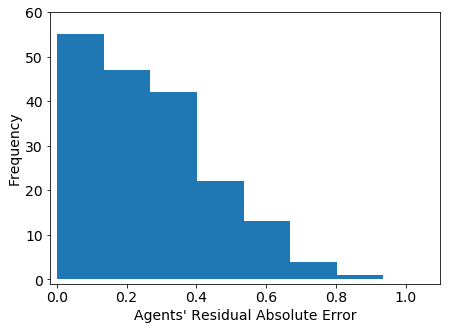
\includegraphics[width=0.45\textwidth]{masters-thesis-master/masters-thesis/contents/04_results/Player_Modeling/Clustering/plots/agents_res_abs_err.png}
%     \label{fig:example_predictions:Agents abs err}
%     }
%   \subfloat[]{
%     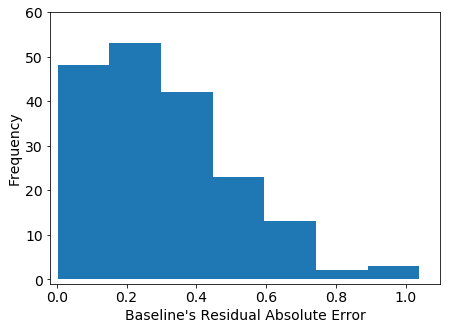
\includegraphics[width=0.45\textwidth]{masters-thesis-master/masters-thesis/contents/04_results/Player_Modeling/Clustering/plots/baseline_res_abs_err.png}
%     \label{fig:example_predictions:Baseline abs err}
%     }
    
%     \caption{Absolute error distributions. Figure (a) illustrates the distribution of the absolute errors for the clustering players approach while Figure (b) illustrates the distribution of the absolute errors for the baseline approach.}
%     \label{fig:abs_err}
% \end{figure}

\subsection*{Predictions using the mean of the players’ success rate}
Regarding data points where the agents or the baseline have a zero \acs{sr}, a prediction is formed using the mean of the players' \acs{sr} where the corresponding agent's or baseline's \acs{sr} are zero in the training data. This means that for each agent, the predictions in the test levels where the agent failed are computed by looking at the mean of the players' \acs{sr} in the training levels where the corresponding agent failed as well. In Table \ref{tab:prediction_performance_tot} we reported both the performance in the linear part and the overall prediction performance. We can say that our approach reduced the MAE by 7\% and the MSE by 4\% when considering both the linear and the mean predictions. Furthermore, we reported the 95\% confidence interval of the measurements. Note that the improvement of our approach is lower when considering the mean predictions as when considering only the linear part.
Since the agents and the baseline failed in different levels, we need to consider that the number of levels predicted with the mean is different between each agent and the baseline. On average the six agents predict 62 levels using the mean while the baseline predicts 69 levels with the mean.
We ran a paired t-test to check that the within pair difference obtained is larger than would be expected to have occurred by chance. Since we obtained a two-tailed p-value greater than 5\% we cannot reject the null hypothesis when considering also the predictions realized with the mean \acs{sr}.
\begin{table}[h!]
    \centering
    \small
    \caption{Clustering players. Regression performance measures} 
       \begin{tabular}{l c c c c }
    \toprule
    
    & \multicolumn{2}{c}{MAE} & \multicolumn{2}{c}{MSE} \\
    % & \multicolumn{2}{c}{Adj R-squared}  \\
    \cmidrule(r){2-3} 
    \cmidrule(r){4-5}

    Approach & Linear part & Total & Linear part & Total  \\
    % & Linear part & Total
    \midrule
    Baseline            & 0.30 $\pm$ 0.03 & 0.31 $\pm$ 0.02 & 0.13 $\pm$ 0.02 & 0.14 $\pm$ 0.02   \\ % & 0.43 & 0.43
    Clustering players  & 0.26 $\pm$ 0.03 & 0.29 $\pm$ 0.02 & 0.10 $\pm$ 0.02 & 0.13 $\pm$ 0.02 \\  % & 0.56 & 0.46 
    
    \bottomrule
    \end{tabular}
    \label{tab:prediction_performance_tot}
\end{table} 

Figure \ref{fig:boxplot_tot} illustrates the distribution of the \acs{sr} for the failed levels of each agent as well as the mean used to predict in these cases. The players' \acs{sr} in the failed levels tend to be lower compared to the succeeded levels. This is desirable since we expect levels where the agents failed to be difficult for the players as well. However, the variance is high and as a consequence the mean prediction performs poorly. Furthermore, since the failed levels represent on average 18\% of the test levels, their impact on the regression performances is considerable. Finally, we can observe that the predicted mean in the baseline approach is closer to the true mean compared to other agents. This is due to the fact that the baseline represents a greater number of players and their average \acs{sr} is less variable between training and test levels. On the contrary, the average \acs{sr} on failed levels for some agents, especially agents 1, 2 and 3, changes a lot between training and test levels. This was expected by looking at the \acs{sr} distribution in Figure \ref{fig:k_means} and it can explain why adding these levels reduces the performances of our approach.

\begin{figure}[h!]       
    \centering
    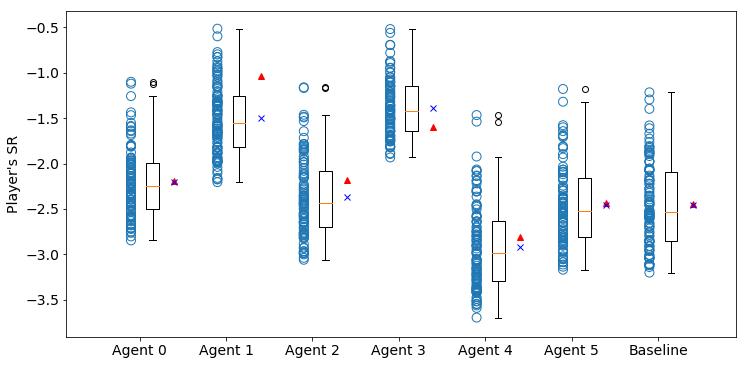
\includegraphics[width=0.6\textwidth]{masters-thesis-master/masters-thesis/contents/04_results/Player_Modeling/Clustering/plots/boxplot_zeros.png}
    \caption{Data points and boxplots of levels predicted with the mean. The red triangles show the mean prediction of each agent while the blue crosses indicated the true mean.}
     \label{fig:boxplot_tot}
\end{figure}

\subsection{Clustering Simulated Strategies Approach}

In this approach, since we cannot accurately determine how many players each agent simulates, instead of combining the predictions of six different linear models, we use a single linear regression model with six predictors.
Another difference with the previous approach is that we no longer need to eliminate levels that drastically changed since both the players' \acs{sr} and the agents' \acs{sr} are computed using the most recent and identical version of the levels.

As we did for the clustering players approach, we validated the four linear regression assumptions in the training data and we reported the plots in Appendix \ref{assamp_val_sim_strategies}. We can observe that the assumptions hold with only a minor violation of the homoscedasticity of the errors assumption. 
Subsequently, we used the linear model fitted with the six agents' \acs{sr} and the one fitted with the baseline's \acs{sr} to predict on test levels. Table \ref{tab:prediction_performance_linear_sim} reports the evaluation of our approach compared to the baseline. The clustering simulated strategies approach reduced the prediction MAE from 0.30 to 0.26 with an improvement of 13\%, the prediction MSE from 0.17 to 0.13 with an improvement of 24\% and finally improved the adjusted R-squared from 0.51 to 0.62 with an improvement of 22\%. 
We ran a paired t-test to check that the per-level mean difference of the absolute errors between the two approaches is different from zero with a significance level of 5\%. We obtained a two-tailed p-value of 0.08\% and rejected the null hypothesis concluding that the mean difference between the two approaches is statistically significantly different to zero.
For completeness, we ran a two-sided t-test to check that the two approaches have a statistically different \acs{MAE}. We obtained a two-tailed p-value lower than 5\% and we rejected the null hypothesis of identical average scores. Furthermore, since in this approach we compared a linear model with six predictors with a linear model with a single predictor, the most important metric is the adjusted R-squared because it takes into account the number of predictors. More precisely, the adjusted R-squared decreases if we add a predictor that improves the model less than what would be improved by chance. 
% Finally, also the standard deviation of the absolute errors is reduced, from $0.25$ for the baseline approach to $0.27$ for the proposed approach.
\begin{table}[h!]
    \centering
    \small
    \caption{Clustering simulated strategies. Overall regression performances} 
       \begin{tabular}{l c c c }
    \toprule
    
    
    Approach & MAE & MSE & Adj R-squared \\ 
    
    \midrule
    Baseline & 0.30 $\pm$ 0.04  & 0.17 $\pm$ 0.06 & 0.51  \\ 
    Clustering simulated strategies & 0.26 $\pm$ 0.03 & 0.13 $\pm$ 0.05 &  0.62 \\ 
    

    \bottomrule
        
    \end{tabular}
    
    
    
    %   \begin{tabular}{l c c c c c}
    % \toprule
    
    % & \multicolumn{2}{c}{MAE} & \multicolumn{2}{c}{MSE} & \\
    % % & \multicolumn{2}{c}{Adj R-squared}  \\
    % \cmidrule(r){2-3} 
    % \cmidrule(r){4-5}
    
    % Approach & Mean & Std err & Mean & Std err & Adj R-squared \\ 
    
    % \midrule
    % Baseline & 0.30 & 0.019 & 0.17 & 0.032 & 0.51  \\ 
    % Clustering simulated strategies & 0.26 & 0.017 & 0.13 & 0.024 &  0.62 \\ 
    

    % \bottomrule
        
    % \end{tabular}
    \label{tab:prediction_performance_linear_sim}
\end{table} 


\subsection*{Predictions using the mean of the players’ success rate}

The data points where any of the agents or the baseline failed are predicted using the mean of the players' \acs{sr} in the training levels where the corresponding agents or baseline failed as well.
In Table \ref{tab:prediction_performance_tot_sim} we reported the prediction performances in the linear part and the overall performances. The six agents predicted 193 levels using the mean since whenever one of the agents failed a mean prediction is applied, on the contrary, the baseline predicted only 101 levels using the mean players' \acs{sr}. Considering all predictions, the clustering simulated strategies approach achieved a 8\% lower MAE, a 16\% lower MSE and a 19\% higher adjusted R-squared than the baseline approach. However, we ran a paired t-test and we obtained a two-tailed p-value greater than 5\%. As a consequence, we cannot reject the null hypothesis of mean difference identical to zero when considering also the predictions realized with the mean \acs{sr} with a significant level of 0.05. 

\begin{table}[h]
    \centering
    \small
    \caption{Clustering simulated strategies. Regression performance measures} 
       \begin{tabular}{l c c c c c c }
    \toprule
    
    & \multicolumn{2}{c}{MAE} & \multicolumn{2}{c}{MSE}  & \multicolumn{2}{c}{Adj R-squared}  \\
    \cmidrule(r){2-3} 
    \cmidrule(r){4-5}
    \cmidrule(r){6-7}

    Approach & Linear part & Total & Linear part & Total & Linear & Total \\
    \midrule
    Baseline            & 0.30 $\pm$ 0.04 & 0.35 $\pm$ 0.03 & 0.17 $\pm$ 0.06 & 0.22 $\pm$ 0.05 & 0.51 & 0.46 \\
    Clustering sim. str.  & 0.26 $\pm$ 0.03 & 0.32 $\pm$ 0.03 & 0.13 $\pm$ 0.05 & 0.18 $\pm$ 0.04 & 0.62 & 0.54 \\
    
    \bottomrule
    \end{tabular}
    
    \label{tab:prediction_performance_tot_sim}
\end{table} 

Note that the performance metrics reported in this thesis are computed on the scaled and log-transformed values. Reverting the \acs{sr} predictions and computing the errors on the original \acs{sr} values only led to different absolute values yet similar improvements between the proposed approaches and the baseline.

\section{Estimating Strategy Requirements}\label{estimate_strategy}

We performed an analysis to categorize levels based on the strategy required to solve them. This approach is built on the assumption that the strategy learnt from player data is enough to solve the levels. Nevertheless, we observed that on average between agents, 82\% of the tested levels are successfully solved. We created a population of 16 different agents, each one simulating a different amount of strategy error. By comparing the performances of the agents, we estimate the strategy required by each level. We randomly selected 20 levels to test this approach and we ordered the agents that use an $\epsilon$-greedy policy from the one that plays completely random (\textit{$\epsilon$ = 1}) to the one that plays greedily (\textit{$\epsilon$ = 0}). By plotting the agent's \acs{sr} against the amount of strategy used, represented by \textit{$1 - \epsilon$}, we observed how the \acs{sr} improves as we reduce the number of random moves made by the agent.
Figure \ref{fig:two_levels_strategy} shows for levels 154 and 155 the strategy level plotted against the agents' \acs{sr}. The strategy level represents the amount of strategy used by the agent. As a consequence a strategy level of zero means that the agent uses a random policy while a strategy level of one means that the agent follows a greedy policy. Note that the agents' \acs{sr} are normalized dividing them by the maximum value. This because in order to compare levels we assume that when the agents play with full strategy they reach the optimal performances ($SR = 1$). To estimate the strategy required by a level, we computed the area above the line. By computing this metric for the two levels in Figure \ref{fig:two_levels_strategy} we obtained a strategy requirement of $0.72$ for level 154 and a strategy requirement of $0.24$ for level 155. 

Finally, Figure \ref{fig:sr_strategy} illustrates the scaled players' \acs{sr} against the strategy required. We scaled the \acs{sr} dividing by the difference between the maximum and the minimum \acs{sr} to not show the actual values for privacy reasons. We observe that the strategy requirement is correlated with the players' \acs{sr}. Although some levels have a similar \acs{sr}, they have significantly different strategy requirements. This indicates that even if two levels have a similar difficulty, the concentration and focus required by players to solve them is different.
\begin{figure}[H]
  \centering
  \subfloat[]{%Level 154
    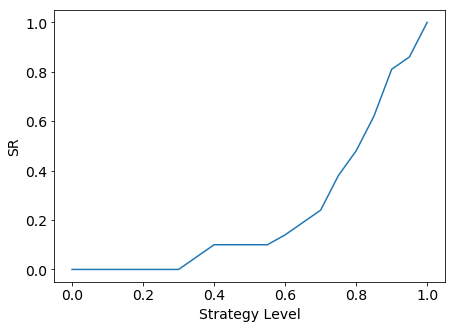
\includegraphics[width=0.45\textwidth]{masters-thesis-master/masters-thesis/contents/05_discussion/strategy_req/154.png}
    \label{fig:154}
    }
    \subfloat[]{%Level 155
    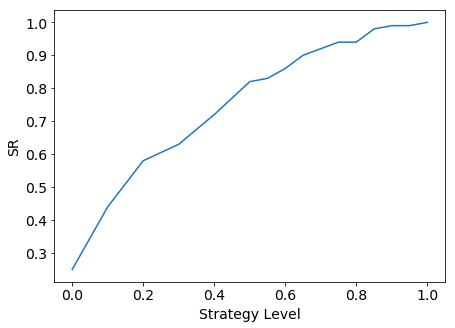
\includegraphics[width=0.45\textwidth]{masters-thesis-master/masters-thesis/contents/05_discussion/strategy_req/155.png}
    \label{fig:155}
    }
    \caption{Two examples of strategy requirement plots for two random levels. Figure (a) shows a level (number 154) that has a high strategy requirement while (b) shows a level (number 155) that requires less strategy to be solved. The \acs{sr} on the y-axis is normalized dividing it by the maximum value.}
    \label{fig:two_levels_strategy}
\end{figure}

\begin{figure}[b]
  \centering
    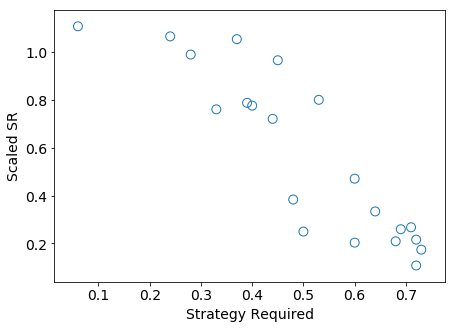
\includegraphics[width=0.45\textwidth]{masters-thesis-master/masters-thesis/contents/05_discussion/strategy_req/sr_strategy.png}
    \caption{Players' \acs{sr} against the strategy required for the 20 different tested levels.}
    \label{fig:sr_strategy}
\end{figure}
We found that \textit{Jelly levels} have on average a higher strategy requirement compared to other types of levels even with a similar \acs{sr}. However, this difference in the strategy requirement is present only on easy levels (with a high players' \acs{sr}). This is explainable by the fact that in order to solve them, the player has to perform the moves above the jelly tiles and performing random moves in other positions reduces the possibilities to clear all the jellies and finishing the level. Regarding more difficult levels, the simple strategy of performing the moves above the jelly tiles is not enough and more complex reasoning is needed. This explains the fact that for difficult levels there is no a clear difference in the strategy requirements between different types of levels. Finally, we can hypothesize that levels that can be successfully solved also with random moves might be perceived less challenging by some players or that levels that require too much strategy might be an obstacle to some other players. A deeper analysis is needed to verify these hypothesis. Furthermore, in the proposed analysis we only uses a single agent and modified it by adding different amount of human errors. In future work we will increase the diversity in the population of developed agents by adding human errors not only to one agent but to all the agents obtained with the two player modeling techniques proposed in this thesis.







